
%%%%%%%%%%%%%%%%%%%%%%% file typeinst.tex %%%%%%%%%%%%%%%%%%%%%%%%%
%
% This is the LaTeX source for the instructions to authors using
% the LaTeX document class 'llncs.cls' for contributions to
% the Lecture Notes in Computer Sciences series.
% http://www.springer.com/lncs       Springer Heidelberg 2006/05/04
%
% It may be used as a template for your own input - copy it
% to a new file with a new name and use it as the basis
% for your article.
%
% NB: the document class 'llncs' has its own and detailed documentation, see
% ftp://ftp.springer.de/data/pubftp/pub/tex/latex/llncs/latex2e/llncsdoc.pdf
%
%%%%%%%%%%%%%%%%%%%%%%%%%%%%%%%%%%%%%%%%%%%%%%%%%%%%%%%%%%%%%%%%%%%


\documentclass[runningheads,a4paper]{llncs}

\usepackage{amssymb}
\setcounter{tocdepth}{3}
\usepackage{graphicx, comment}

\usepackage{url}
\urldef{\mailsa}\path|stuetzlec@merrimack.edu|
\urldef{\mailsb}\path|sammat@rpi.edu|
\urldef{\mailsc}\path|cutler@cs.rpi.edu|
% }@springer.com|    
\newcommand{\keywords}[1]{\par\addvspace\baselineskip
\noindent\keywordname\enspace\ignorespaces#1}

\begin{document}

\mainmatter  % start of an individual contribution

% first the title is needed
\title{
%
Multimedia Groupware for Graph \\ Interaction and Visualization\\
\vspace{-0.1in}
%
}

% a short form should be given in case it is too long for the running head
\titlerunning{ }

% the name(s) of the author(s) follow(s) next
%
% NB: Chinese authors should write their first names(s) in front of
% their surnames. This ensures that the names appear correctly in
% the running heads and the author index.
%
\author{ 
Christopher Stuetzle
\and Tyler Sammann
\and Barbara Cutler }
%
\authorrunning{}
% (feature abused for this document to repeat the title also on left hand pages)


% the affiliations are given next; don't give your e-mail address
% unless you accept that it will be published
\institute{
% Rensselaer Polytechnic Institute\\
% 110 8th St. \\
% Troy, NY 12180 \\
\mailsa \hspace{0.1in}
\mailsb \hspace{0.1in}
\mailsc 
\vspace{-0.2in}
}

%
% NB: a more complex sample for affiliations and the mapping to the
% corresponding authors can be found in the file "llncs.dem"
% (search for the string "\mainmatter" where a contribution starts).
% "llncs.dem" accompanies the document class "llncs.cls".
%

\toctitle{ }
\tocauthor{}
\maketitle


\begin{abstract}
We present a system for developing multi-user, multi-cursor, multi-media, single display groupware that allows for
intuitive interaction with visual graph datasets. 
%The system allows for a variety
%of input device types to work together to produce user input. 
%Several applications
%have been developed 
Our software
%using this 
framework 
%that 
separates the application and the input
device modules with
%through 
an interface that handles generic {\em gestures} captured from
%produced by
different input devices.
% 
The system's gesture set was designed to handle 
standard actions for graph data interaction.
% 
% including USB mice and laser pointers.
% and delivers pertinent information to the application itself, which needs
%no information about the type of device creating the input. 
To enhance the collaborative group interaction experience
for ease of graph data exploration, 
we present an automatic method for adjusting the global focus and zoom level.
%ing We also present the idea of
%crop zooming, a method for focusing the display on the data near the user's cursors
%while still allowing free movement throughout the data visualization. 
Our system allows simultaneous input from works for multiple USB mice
and laser pointers.  To utilize laser pointers as input devices, we
also present the idea of a persistent \textit{laser personality}
of its infrared leak.
%.  By
%identifying an inexpensive, off-the-shelf laser pointer by its
%infrared leak, we are able to uniquely identify any laser used in the
%system with no modifications to the laser pointers, thus treating them
%like generic cursors to interact with our application interface. 
Our 
%The
system is extensible and scalable due to its heavy emphasis on
modularity, and works on both single output screens and large-scale
projection surfaces.
% \fbox{add more on graph interaction \& graph visualization...??}
\vspace{-0.1in}
\end{abstract}

%%%%%%%%%%%%%%%%%%%%%%%%%%%%%%%%%%%%%%%%%%%%%%%%%%%%%%%%
\section{Introduction}

%\vspace{-0.1in}


\begin{figure}[t]
 \centering
 \includegraphics[width=0.62\textwidth]{images/synenv_images/cs_students_4.jpg}
 \includegraphics[width=0.372\textwidth]{images/synenv_square.jpg}%
\vspace{-0.1in}
 \caption{\label{figure:using_mice_and_lasers} Our system supports
   collaboration between multiple users that are using individual USB
   computer mice or green presentations lasers to
   simultaneously interact with graph data visualization.
%  blah blah
% The GUI on the left allows users to select 
% which nodes are visible, as well as select actions to take (bottom left corner) between point, select, pan, 
% and draw. Selecting a node enlarges it to display the data found within, while panning moves the camera around 
% the map. Draw allows the user to make annotations to the visualization, for the benefit of other users. }
\vspace{-0.1in}
}
\end{figure}


Implementing multi-user interaction with node-based data
% is a necessary and well-established 
% research goal
% that 
presents a challenging and worthwhile design problem.
Whether it be in a classroom or a war-room, on a small monitor or a large-scale projection surface,
it is important that groupware (software that takes input from multiple devices and users at once)
systems be developed
that allow for multiple users to efficiently and intuitively interact with and explore
node-based visual datasets.
The design of such a system must consider
what data the users see,
% challenges as far as how much data
and how each user understands what cursor she is controlling.
%they are controlling
% the users can see,
% what objects in the system each user is controlling,
% % at any particular point in time, 
% and what data is valuable and important to showcase.
% 

Groupware with multiple user-controlled cursors has been used for this
% educational 
purpose before, especially
in lower-income or developing areas
where it is cost prohibitive to provide sufficiently many computers for individual use
\cite{Pawar2006,Pawar2007} and student-to-computer ratios suffer.
%the relatively high cost of computers, there is a
% severe lack of computer availability in the educational systems of
% developing nations. 
% \fbox{tell me more about the purpose/functionality of these interfaces}
% In many environments, students in a collaborative learning environment
% are often sharing a single desktop, or screen. 
% By allowing multiple 
% pointers of various device types, an application can provide for many users to
% interact with data.
Classroom environments provide a compelling example for the benefit of 
groupware systems, in which several students learn to
solve problems in a collaborative manner through educational software,
allowing for collaborative problem solving exercises, data exploration,
and visualization software to be used.
In general, collaborative problem solving software can be useful in a variety of situations,
including emergency response, educational software, data exploration and manipulation,
land planning and flood mapping, etc.

%
% This idea need not be limited to single computer kiosks. 
% It is important to 
Many classrooms are now equipped with large-scale projection surfaces
to facilitate lesson plans.
The growing prevalence of 
% a variety of 
various output devices
has created the need for software allowing users to interact with a range of
displays, from single computer screens to large-scale projection
surfaces. 
% provides more flexibility in groupware design.  
% Therefore, a system that caters to both a variety of output
% and input devices by allowing for easy customization is preferable .
% to ones that do not.
% \fbox{paragraph is vague}

We have designed a system for node-based data interaction for multiple
users utilizing a variety of input device types
% (e.g., mice, laser pointers, or 3D imaging for gesture tracking) 
that can be used with a
variety of output devices (e.g., PC monitors or large-scale projection
surfaces).  Our system provides a modular
%ity-dependent 
software framework that separates the {\em cursors} (general pointing
and interaction devices) from the computer application. This is
accomplished by a well-defined set of {\em gestures} that can be 
% created
detected by each of the input cursors and customized by the
application as needed.
% These cursors can range from mice to laser pointers to the Microsoft Kinect, and anything in between.
%\fbox{add back in kinect mention?}

\vspace{0.1in}

\noindent
Our contributions are:

\begin{itemize}
 \item an extensible and intuitive system for interacting with node-based datasets, on either a small screen or a large-scale display,
 \item an interface allowing for collaborative data exploration through several different input media simultaneously,
 \item a novel focus and zooming procedure based on the current cursor positions of users, and
%for exploration focused only on what users are currently viewing.
 \item consistent identification of the \emph{laser pointer personality}, the signature shape and intensity of a laser point's infrared light leak.
% and a system that uses it to uniquely identify inexpensive, off-the-shelf laser pointers.
\end{itemize}

In addition to specific contributions, there are several advantages to our approach. 
The system is scalable to large datasets
% , and works with large datasets, both spatial and relative.
%In addition, it 
and provides functionality for a large variety of gestures,
and it is 
%, and more can easily be added. 
% The system is 
designed with a modular and extensible API that allows a great deal of flexibility by the application,
but leaves the device handling behind-the-scenes. 
% Since all devices are treated as ``cursors'', an application
% using the system does not have knowledge of each individual input medium, and instead simply provides reactions
% to various input gestures.


%%%%%%%%%%%%%%%%%%%%%%%%%%%%%%%%%%%%%%%%%%%%%%%%%%%%%%%%
\section{Related Work in Groupware Implementation}

% Our system is currently designed for handling two popular input media: mice and laser pointers.

%----------------------------
\paragraph{\bf Multiple Mice}

Interfaces utilizing multiple mice cursors on a single output screen
have existed for many years.  A computer mouse is a classic, cheap,
widely understood, functionally simple, and robust user input device,
making it the preferred human input device when multi-user interaction
was first conceptualized.
 
Bier et al. describe a system built for multiple users and a single
display, using a mouse for each user, and individual cursors for each
mouse~\cite{Bier1991}.  The system
%presented 
allows for dynamic creation of new {\em user instances}, each assigned
an individual {\em home area}. 
% Input events from the mice are handled
% with an event record
% queuing data structure that stores time stamp, as
% well as device ID and state information.
% The toy application built around the system was functionally very
% simple, but provided proof of concept for such a system, and introduced
% important multi-user interface elements. Such elements included the distinction
% of cursors based on color, and interface elements (windows) with nested scopes,
% allowing for parent-child management relations between elements, and element
% ``ownership.''
%
% Sample applications for the systems that followed were often functionally
% simple. 
Stewart et al. present applications for their own multi-cursor single
display architecture, coining the term {\em single display groupware}
(SDG)~\cite{Stewart1999}.  They enumerate potential benefits of a
SDG paradigm, the most notable being the enrichment of existing
computer collaboration, and the ability for learning and teaching
% scenarios between users. One application for their system
%, named 
%{\em  KIDPAD}, 
% allowed multiple users to draw simultaneously.
% The application
% presented the notion that each user have the ability to select their own local
% tool (like a paintbrush) to make edits to the drawing. One of the tools
% available allowed for the removal of changes made by a particular user,
% furthering the concept of locality and ownership in the application.
%
% Though modern operating systems are capable of handling input from
% multiple mice simultaneously, this does not result in the respective
% number of individual operating system level cursors appearing on
% the screen. Rather, every participating device controls the same
% single cursor.  
Pawar et al. discuss 
% this issue, 
the problem that an operating system is unable to provide
more than one OS-level mouse cursor,
and resolve it by
suppressing the primary (operating system) mouse cursor, and
displaying custom multi-mouse cursors within the application
itself~\cite{Pawar2006}.
% Because the Win32 API
% in Windows XP ignores the unique identifiers given to each USB mouse, they
% utilize the RawInput API in Windows XP, which gives them access to data-rich
% mouse data including unique IDs, as well as callback access for each of the
% mice. 
Pawar et al. present a second study using the same architecture for
multiple mice, and more conclusively prove the failings of a
system with multiple users and a single cursor~\cite{Pawar2007}.
% 
% The applications presented by Pawar et al. took the SDG paradigm into the
% educational domain. 
% Due to the high cost of computers, there is a
% severe lack of computer availability in the educational systems of
% developing nations.   
% ... moved some of this text earlier...
The SDG paradigm was 
taken into the educational domain and 
used to create applications that
extend the educational and collaborative effectiveness of one computer by
allowing simultaneous users with cheap USB mice~\cite{Pawar2006}. 
% A later study
% showed the educational advantages and disadvantages to having strictly
% competitive applications and strictly collaborative applications. It was
% demonstrated that learning retention is much higher in a collaborative setting
% than a competitive one. This was especially true with groups of
% boys~\cite{Pawar2007}.

% \subsubsection{Laser Pointers}

\vspace{-0.15in}
%----------------------------
\paragraph{\bf Laser Pointers}
For large group interaction with a single display, 
% a standard computer
% monitor is insufficient.  
large-scale projection displays are preferable to monitors,
and the use of a standard presentation laser pointer as a
cursor is a cost-effective mechanism to support group interaction with
the presentation.
%In large-scale Laser pointers are used exclusively for large-scale display interaction.
There are two steps to using laser pointers as an input medium on such
a display.  First, each active laser spot must be detected, and
second each spot must be identified, tracked, and associated
with
% a history of actions for that 
a particular cursor/user.

Single laser point detection is accomplished in two main ways:
brightness filtering and infrared filtering.  Olsen and Nelson detect
a laser spot on a large display screen with a two pass
system~\cite{olsen2001}.  The first pass detects the brightest red
spot in the image, while the second 
% (which only occurs if no obvious laser spot is found) 
% passes over the screen again, employing a
% convolution filter, concentrating 
employs a convolution filter 
on the area where the last spot was
detected.  Oh and Stuerzlinger allow for multiple laser points by
applying a threshold to the brightness field of the
image~\cite{Oh02laserpointers}.  The same technique is applied by Davis
and Chen in their LumiPoint system~\cite{Davis00lumipoint:multi-user}.
% However, depending on the
% brightness of the laser spot with respect to the rest of the image can
% create trouble, as it is context sensitive and simple thresholds may
% confuse the laser points and very bright sections of the
% image. 
Ahlborn et al.~\cite{Ahlborn:2005:PSL:1101616.1101637} present a
system using multiple camera views in which the background image is
filtered out leaving only laser points for detection.  If the laser
pointers include IR spectrum light, an IR pass filter 
will
%can be used to
ignore the visible light from the projector and focus on the
invisible-to-humans IR dot for each laser.  IR filtering is employed
by work by Qin et al.~\cite{Qin:2010:SLP:1842993.1843022}, Angelini et
al.~\cite{angelini:multi-user}, and Cheng et
al.~\cite{Cheng:2003:DIL:857080.857088}.
%
Laser pointer identification is the second and more challenging step.
One method is to
dynamically change the number of lasers present in the system at any
given point in time, and to track an IDed laser spot across frames
with predictive measures, such as the Kalman
filter~\cite{Oh02laserpointers,Davis00lumipoint:multi-user,Cheng:2003:DIL:857080.857088}.
%
% \fbox{THE LAST SENTENCE MAKES NO SENSE TO ME...  HOW DO THEY DO THIS?  DID THIS DESCRIPTION GET MANGLED?}
%
Another method involves the use of time division multiplexing, or the
 application of a laser blinking pattern, to identify a particular
 laser~\cite{Vogt:2004:ECG:1009379.1009663,Vogt03trackingmultiple,Pavlovych04laserpointers}.
% 
Given \emph{n} lasers, a system can force exactly one of the
lasers off each frame,
and at high enough frame rates the ID of a laser spot can be determined by the frames its spot is missing.
% With cameras with high frame rates, this
% produces an unnoticeable effect with regard to the temporal coherence
% of the laser spot on the screen, but the system can identify the laser
% by its blinking pattern. 
% This method is 
%as employed by Vogt et
%al.~\cite{Vogt:2004:ECG:1009379.1009663,Vogt03trackingmultiple}, as
%well as Pavlovych and Stuerzlinger~\cite{Pavlovych04laserpointers}.


% Laser point detection, both single- and multi-user, has a variety of
% applications, most of which revolve around user collaboration and
% interaction. Francisco de la O Chavez et al., present a system
% whereby users can operate the electronic devices and appliances in
% their homes with a laser pointer~\cite{delaOChavez:2008:INL:1387269.1387276}. The system uses a
% single camera, and the user sets up ``active zones'', or groups of
% pixels in the camera view around each appliance. When a laser spot is
% detected in the active zone, the appliance is activated. Qin et al.,
% present a system in which a special laser pointer is used to project
% several beams, and the orientation of the beams indicates the angle of
% rotation along the beam axis of the laser, thus allowing for gestures
% and object manipulation that involves rotation~\cite{Qin:2010:SLP:1842993.1843022}. Bi et al. present the uPen, a
% laser pointer outfitted with right- and left-click buttons, designed
% to mimic computer mouse functionality~\cite{BiUpen}.
% Shizuki et al.~\cite{Shizuki:2006:LPI:1133265.1133284} present a series of 
% gestures used with a laser pointer, and a series of applications using them.
% The gestures are edge-crossing gestures, and the applications presented include 
% a presentation application using gestures to move slides forward, and a picture 
% viewing application where gestures manipulate the images.

% \vspace{0.1in}


% \fbox{buzzwordify: ``unify'' the interface?}

\vspace{-0.1in}
%----------------------------
\paragraph{\bf Image-Based 3D Scanning Gesture Tracking}
% \fbox{write discussion of Kinect \& Leap Motion, steal from later text??}

Many products are being released that use image-based 3D scanning to track 
user
gestures and movement.
% in both small- and large-scale settings. 
One example is the Microsoft Kinect peripheral for the Microsoft XBox 360
game console
% , for which games are designed that read the players'
% gestures as input 
\cite{Kinect}.
A similar technology, introduced by Leap Motion, Inc. for use with Microsoft's 
Windows OS, is Leap Motion,
% which has a significantly higher resolution 
which is more sensitive
than the Kinect \cite{LeapMotion}.
Small motions, such as hand squeezes and finger clicks, are detected and used 
by the OS in lieu of a mouse.

To our knowledge, no prior work has 
%been published regarding the
% % identification of off-the-shelf laser pointers in multi-user
% % applications.
% % Also, the domain of applications that have been explored
% % for multi-user laser pointer interaction is rather small, either due
% % to lack of need or due to the necessity of engineering laser pointers
% % to make the interfaces effective.
unified
%cation of 
multiple input media for collaborative problem solving and 
graph data exploration groupware. 
% In addition, the identification of off-the-shelf laser pointers in multi-user
% applications is a novel contribution.

\vspace{-0.1in}
%%%%%%%%%%%%%%%%%%%%%%%%%%%%%%%%%%%%%%%%%%%%%%%%%%%%%%%%
\section{Interaction Interface}
\vspace{-0.1in}

\begin{figure}[t]
 \centering
%  \includegraphics[width=0.49\textwidth]{images/Baby_Food_NoExpand.png}
\includegraphics[height=0.28\textwidth]{images/group_select_A.png}\hfill%
\includegraphics[height=0.28\textwidth]{images/group_select_B.png}\hfill%
\includegraphics[height=0.28\textwidth]{images/group_select_C.png}\hfill%
\includegraphics[height=0.28\textwidth]{images/group_select_D.png}%
% \includegraphics[width=0.49\textwidth]{images/Baby_Food_TwoExpand.png} 
%  \vspace{0.05in}
% \includegraphics[width=0.49\textwidth]{images/Baby_Food_GroupAction.png}%
%  \includegraphics[width=0.49\textwidth]{images/Baby_Food_ChocolateVsFood.png}
\vspace{-0.1in}
 \caption{\label{figure:gesture_select_move_group_expand_simplify} 
Exploring the animal
   classification hierarchy dataset, the user first {\em selects} five nodes and
   performs the {\em group} action.  Then the user perform an {\em expand}
   operation on the group which expands the graph to include expands
   of animals within each category and display the associated images.
   Next the user {\em simplifies/collapses} the portion of the tree containing the
   invertebrates.  Finally, the user increases the size of several
   images and {\em moves} some of the nodes to rearrange the graph layout.
\vspace{-0.1in}
}
\end{figure}



% \begin{figure}[t]
%  \centering
% % \includegraphics[width=0.49\textwidth]{images/AnimalsScreenshot2_NoGrayBox_NoZoom.png}
%  \includegraphics[width=0.49\textwidth]{images/AnimalsScreenshot3_GrayBox_NoZoom.png}
%  \includegraphics[width=0.49\textwidth]{images/AnimalsScreenshot4_GrayBox_Zoom.png}
%  \caption{\label{figure:crop_zoom} A visualization of our graph exploration application, in which a 
% database with connectivity information is read in, displayed, and explored by users. In this instance, the data 
% used is a taxonomic tree of animals. These three images demonstrate the crop zooming option of our
% system. Image a) shows the visualization with no annotations. A gray box is displayed in image b), outlining
% the bounding box of the user's cursors. Finally, image c) provides the view when crop zooming is 
% activated, and the view is cropped to only around the user pointers, plus a small buffer zone. }
% \end{figure}


Our modular software design separates the application from the exact media of the user input devices.
%application architecture separates the design of software into a set of device modules
%that are controlled through an interface.
%The interface acts as a middleman between the input devices and an application designed to use them by 
%treating each input device type as a separate module that provides input data for categorization.
The application is presented an interface to generic cursors,
and
%Any application using the system needs no knowledge of the device types, and instead simply treats
%every device as a {\em cursor}.
%
% The interface 
registers {\em callbacks} 
% with the cursor managing interface 
to receive and handle the different {\em gestures} detected
from each
% different
input device.
%regularly checks input data from the modules for the
%presence of any one of a series of predefined {\em gestures} that are
%used to interact with the application.  
Each gesture is passed to the application along with the ID of the cursor making the gesture.
%When a gesture is detected by
%the interface, the application is informed of the gesture and the
%cursor that made it.  
For example, if one of the device types is a
mouse, and the user left-clicks with it, the interface informs the
application that a {\em select} gesture has been issued, along with the
particular cursor that made the gesture.
% 
This framework creates a single layer of abstraction between the input
devices and the application 
%(similar to the way an operating system
%acts) 
that allows for clean, easy-to-debug application development.


\begin{figure}[t]
 \centering
  \includegraphics[width=0.24\textwidth]{images/graph_interaction_A_smaller.png}\hfill%
  \includegraphics[width=0.24\textwidth]{images/graph_interaction_B_smaller.png}\hfill%
  \includegraphics[width=0.24\textwidth]{images/graph_interaction_C_smaller.png}\hfill%
  \includegraphics[width=0.24\textwidth]{images/graph_interaction_D_smaller.png}%
\vspace{-0.1in}
 \caption{\label{figure:graph_interaction} Users exploring a dataset
   of 25,000 images from Flickr~\cite{MIRFLICKR}.  Each image is
   tagged with a number of descriptive strings.  The application
   launches with some of the more common tags.  First, the users
   simplify/collapse some of the less interesting tags (e.g.,
   ``Nikon'', ``explore'') and manually arrange some of the key nodes
   in the graph structure for clarity.  Then they begin exploring the
   available images and zoom in on a portion of the graph.
\vspace{-0.1in}
}
%Screen shots taken from our graph interaction application. 
%  A) Two datasets on the screen, full collapsed. 
% On the left, the data after several {\em expand} gestures in which nodes expand to show 
% their adjacencies. 
% On the right, the {\em group} action, in which two nodes have been grouped together and are controlled
% by the yellow mouse, moving together.  \fbox{FIGURE SHOWING EXPAND \& SIMPLIFY}
\end{figure}




\vspace{-0.1in}
%----------------------------
\paragraph{\bf Cursor Gestures}

The system relies on a series of well-defined gestures that can be
created using actions by each of the input device types. For instance,
a generic {\em select} gesture would be a left-click on a standard
mouse, or a hover action by a laser pointer.
%
Each of these gestures is helpful and intuitive for collaborative graph visualization and exploration
%can be considered common and useful for graph
%interaction, 
and developers of other collaborative applications can pick and choose
which gestures to utilize in the application.
% 
Table \ref{table:gestures} contains each gesture recognized by our
multimedia groupware interface, and the associated callbacks triggered
by each input device type.  More complicated gestures can be achieved
by combining those mentioned above
% For instance, 
(e.g., a standard
click-and-drag gesture is simply a combination of select, move, and
release).

Adding more device types is straightforward, and applications that have been designed using the system
do not have to be updated to reflect changes made to the devices.
% 
Any input device can act as a
cursor in the system, as long as it has an on-screen location and a series of states that can be used to 
detect the gestures. 
For example, the final column of Table \ref{table:gestures} outlines a possible mapping of gestures using real-time 3D imaging
scanner such as the Microsoft Kinect or the Leap Motion.  
% \fbox {ADD REFERENCES} \fbox {maybe move some of this earlier...} 
While we have not implemented this module, 
%this module has not
%yet been implemented, 
we include this proposal
%it is provided here for the purpose of
as an example of the extensibility of our system design.
In addition to these, we envision systems that are able to incorporate
eye tracking,
% mind tracking,
keyboards,
stop-motion capture,
or blue tooth devices (such as smart phones)
as input modules.




This gesture set represents a preliminary attempt to capture the most
useful and intuitive user actions on graph data. A user study will be
performed to determine where improvements to the set can be made,
including if any gestures are extraneous or are missing.



% % \paragraph{\bf Extensibility}
% % \fbox{could cut?  or merge with kinect discussion better, how many more device types do we really envision???}
% Adding more device types is straightforward, and applications that have been designed using the system
% do not have to be updated to reflect changes made to the devices. Any input device can act as a
% cursor in the system, as long as it has an on-screen location and a series of states that can be used to 
% detect the gestures. 
% % 
% % The system is currently configured to take input from laser pointers and multi-mice.
% Due to its modular nature, creating a new input device module is a simple step.
% % Creating a module for the Microsoft Kinect, for instance, requires configuring a piece of software
% % to listen to the input from the Kinect (similar to the way the operating system listens for 
% % input information from the Primary Mouse), and recognizing each of the gestures built into the 
% % system from input. 



% \fbox{maybe instead talk about how easy it is to develop a new application to use this interface and to customize the gestures}
% \fbox{CS: I mention above how applications don't need to be updated as devices are added, and mention elsewhere that the application is oblivious to the devices.}

\begin{table}[t]
 \begin{center}
 \begin{tabular}{| l | l | l | l | l |} 
  \hline
  \textbf{Gesture} & \textbf{Description} & \textbf{Mouse} & \textbf{Laser Pointer} & \textbf{Kinect/Leap} \\
  \hline
  \begin{tiny}Select               \end{tiny}&\begin{tiny}Select/Grab an object\end{tiny}&\begin{tiny}Left-Click Down\end{tiny}&\begin{tiny}Hover         \end{tiny}&\begin{tiny}Close fist       \end{tiny}\vspace{-0.05in}\\
  \begin{tiny}                     \end{tiny}&\begin{tiny}on the screen        \end{tiny}&\begin{tiny}               \end{tiny}&\begin{tiny}              \end{tiny}&\begin{tiny}                 \end{tiny}\vspace{-0.02in}\\ \hline
  \begin{tiny}Move                 \end{tiny}&\begin{tiny}Move a cursor or     \end{tiny}&\begin{tiny}Move           \end{tiny}&\begin{tiny}Move while on \end{tiny}&\begin{tiny}Move fist        \end{tiny}\vspace{-0.05in}\\
  \begin{tiny}                     \end{tiny}&\begin{tiny}selected object      \end{tiny}&\begin{tiny}               \end{tiny}&\begin{tiny}              \end{tiny}&\begin{tiny}                 \end{tiny}\vspace{-0.02in}\\ \hline
  \begin{tiny}Release              \end{tiny}&\begin{tiny}Release a selected   \end{tiny}&\begin{tiny}Left-Click Up  \end{tiny}&\begin{tiny}Turn off laser\end{tiny}&\begin{tiny}Open fist        \end{tiny}\vspace{-0.05in}\\
  \begin{tiny}                     \end{tiny}&\begin{tiny}object               \end{tiny}&\begin{tiny}               \end{tiny}&\begin{tiny}              \end{tiny}&\begin{tiny}                 \end{tiny}\vspace{-0.02in}\\ \hline
  \begin{tiny}Simplify             \end{tiny}&\begin{tiny}Reduce the amount    \end{tiny}&\begin{tiny}Right-Click Up \end{tiny}&\begin{tiny}Scribble      \end{tiny}&\begin{tiny}Finger-tap       \end{tiny}\vspace{-0.05in}\\
  \begin{tiny}                     \end{tiny}&\begin{tiny}of visible data      \end{tiny}&\begin{tiny}               \end{tiny}&\begin{tiny}              \end{tiny}&\begin{tiny}                 \end{tiny}\vspace{-0.02in}\\ \hline
  \begin{tiny}Expand               \end{tiny}&\begin{tiny}Increase the amount  \end{tiny}&\begin{tiny}Double-Click   \end{tiny}&\begin{tiny}Circle        \end{tiny}&\begin{tiny}Double finger-tap\end{tiny}\vspace{-0.05in}\\
  \begin{tiny}                     \end{tiny}&\begin{tiny}of visible data      \end{tiny}&\begin{tiny}               \end{tiny}&\begin{tiny}              \end{tiny}&\begin{tiny}                 \end{tiny}\vspace{-0.02in}\\ \hline
  \begin{tiny}Enter/Exit Group Mode\end{tiny}&\begin{tiny}                     \end{tiny}&\begin{tiny}Left-click away\end{tiny}&\begin{tiny}Hover away    \end{tiny}&\begin{tiny}Swipe left       \end{tiny}\vspace{-0.05in}\\
  \begin{tiny}                     \end{tiny}&\begin{tiny}                     \end{tiny}&\begin{tiny}from data      \end{tiny}&\begin{tiny}              \end{tiny}&\begin{tiny}                 \end{tiny}\vspace{-0.02in}\\ \hline
  \begin{tiny}Group                \end{tiny}&\begin{tiny}Group objects        \end{tiny}&\begin{tiny}Left-Click     \end{tiny}&\begin{tiny}Circle        \end{tiny}&\begin{tiny}Close fist       \end{tiny}\vspace{-0.05in}\\
  \begin{tiny}                     \end{tiny}&\begin{tiny}together             \end{tiny}&\begin{tiny}               \end{tiny}&\begin{tiny}              \end{tiny}&\begin{tiny}                 \end{tiny}\vspace{-0.02in}\\ \hline
  \begin{tiny}Ungroup              \end{tiny}&\begin{tiny}Undo grouping        \end{tiny}&\begin{tiny}Right-Click    \end{tiny}&\begin{tiny}Scribble      \end{tiny}&\begin{tiny}Open fist        \end{tiny}\vspace{-0.05in}\\
  \begin{tiny}                     \end{tiny}&\begin{tiny}of objects           \end{tiny}&\begin{tiny}               \end{tiny}&\begin{tiny}              \end{tiny}&\begin{tiny}                 \end{tiny}\vspace{-0.02in}\\ \hline
 \end{tabular}
 \end{center}%
\vspace{-0.1in}
 \caption{
%
\label{table:gestures} 
%
Common gestures for the mouse, laser pointer, and 3D imaging
devices. 
%Each of the gestures is recognized by the interface and
%application is informed of the cursor that made the gesture and what
%the gesture was. 
%The reaction to the gesture is handled by the
%application itself.  Note that Group and Ungroup actions are only
%detected while the cursors are in {\em Group Mode} (GM).
%
% \newline
%  *Gestures in the last two rows occur during .
%
% \fbox{ I don't like the asterisks...  if anything, the asterisks should be used for the interface we did not implement (3D detection gestures image based whatever)}
% \fbox{ also, i wish we could redo so that group isn't a separate mode, but a fluid gesture type...  special modes are annoying to learn}
%
\vspace{-0.1in}
}
\end{table}

%%%%%%%%%%%%%%%%%%%%%%%%%%%%%%%%%%%%%%%%%%%%%%%%%%%%%%%%
\section{Graph Interactions}
\label{section:graph_interactions}


We apply the gestures described above 
%can be applied in a straightforward
%manner 
to various
% standard 
graph visualization applications.
%challenges.  
We demonstrate these gestures on a small tree dataset showing the
animal classification hierarchy, a graph dataset of images and tags
downloaded from 
% \fbox{ADD REFERENCE} 
Flickr~\cite{MIRFLICKR}, and a
spatial dataset of utility infrastructure for a county on the North
Carolina coast.


\begin{figure}[t]
 \centering
 \includegraphics[width=1.0\textwidth]{images/synenv_images/map_screenshot.png}%
\vspace{-0.1in}
 \caption{\label{figure:edge_visualization}
A visualization of our infrastructure data exploration and editing tool.
% that 
% demonstrates two users interacting with the map's data. 
\vspace{-0.1in}
}
\end{figure}

\vspace{-0.1in}
%----------------------------
\paragraph{\bf Visibility \& Information Display}
All of these datasets are large enough that they must be simplified
for legible display on a single standard computer monitor.  When the
visualization is first launched, only a small number of nodes are
tagged as visible.  Only the visible graph nodes are drawn and only
edges between two visible nodes are drawn.
%
In our sample applications, the graph nodes contain varying amounts
and types of information.  Some nodes consist of just a word or two of
text (e.g., animal classification terms), while other nodes contain
numerical data (e.g., utility status, physical location address, etc.)
Some nodes include a symbol or image that can be displayed to enrich
the visualization.  Nodes with complex information can be visualized
in multiple levels of detail (not visible, text only, small
symbol/image, or large image).

For some datasets, the edge linking two nodes may itself contain
important information.  The utility monitoring application shown in
Fig.~\ref{figure:edge_visualization} includes the operational/damage
status for each link between nodes.  We can toggle this extra
visualization by {\em expanding} this edge which thickens the line and
draws text along the path.  For the utility dataset, some of these
edges have complex paths and even lengthy text can be neatly presented
by wrapping it along the path.  To understand the source of a problem
in the utility network, users must work together to investigate
problems at the nodes or edges in this interdependent network.

\vspace{-0.1in}
%----------------------------
\paragraph{\bf Expand/Simplify}
When node $n$ in a tree is targeted by the {\em expand} gesture, the
tree hierarchy is searched starting at that node and working toward
the tree leaves looking for {\em closest} node(s) that are not
currently visible.  All non-visible nodes that are the same distance
(\# of edge links) from $n$ are made visible.  Repeated {\em expand}
operations on nodes with multiple levels of detail (e.g., image data)
will increase the visualization mode of that node to display more
information.  
% The transitions between image sizes are animated to
% create a smooth and dynamic graph visualization.  
Similarly, when a
node is targeted by a {\em simplify} gesture, the tree is searched for
the visible descendant that is furthest from $n$.  All nodes at that
same distance from $n$ are simplified.  First, the complexity level of
the visualization is decreased.  If the node is already at the
simplest level it is made invisible.  For general graphs, without a
clear hierarchy (e.g., a tagged image dataset), the Expand operation
will make visible all nodes connected with a single edge to the
expanded node.  See Figs.~\ref{figure:gesture_select_move_group_expand_simplify}~and~\ref{figure:graph_interaction}.
\vspace{-0.1in}
%----------------------------
\paragraph{\bf Mass Spring Graph Visualization}
For datasets without a strict spatial embedding, we use a simple mass
and spring system to automatically organize the node and edge data.
Each visible node is pulled/pushed by visible graph edges of
neighboring nodes that are also visible.  The rest length for each
visible spring aims to keep the nodes close enough to clearly
represent connectivity, but also far enough to minimize overlap and
allow each nodes text or image data to be clearly represented.  In
abstract graph datasets the users can interactively re-arrange the
data to improve the layout for their needs.
Fig.~\ref{figure:gesture_select_move_group_expand_simplify} shows how the nodes can be {\em
  selected}, {\em dragged}, and {\em grouped}.  
%
% \fbox{WRITE MORE ON GROUPING??}

Nodes that are grouped act as a single object. For instance, dragging
any node causes all nodes within its group to be dragged as well.
% , and
% expanding a node in a group expands all nodes in that group.
Because groups become interactable objects, a natural hierarchy develops
when groups become grouped with other objects, and actions performed
on one recurse down the hierarchy.
% , affecting all objects in the subtree.
% For instance, nodes A and B are grouped into group G1, which is then
% grouped with node C. When A is dragged, so is B. When C is dragged,
% both A and B are as well because they belong to G1, grouped with C. 
Ungrouping inverts the grouping action for all
objects at a single hierarchy level (since nodes exist on exactly one level).

\begin{figure}[t]
 \centering
% \includegraphics[width=0.49\textwidth]{images/AnimalsScreenshot2_NoGrayBox_NoZoom.png}
% \includegraphics[width=0.49\textwidth]{images/AnimalsScreenshot3_GrayBox_NoZoom.png}
% \includegraphics[width=0.49\textwidth]{images/AnimalsScreenshot4_GrayBox_Zoom.png}%
% \includegraphics[width=0.33\textwidth]{images/auto_zoom_A.png}\hfill%
% \includegraphics[width=0.33\textwidth]{images/auto_zoom_B.png}\hfill%
% \includegraphics[width=0.33\textwidth]{images/auto_zoom_C.png}%


 \includegraphics[width=0.29\textwidth]{images/autozoom_full_large_red_scaled.png}\hfill%
 \includegraphics[width=0.29\textwidth]{images/autozoom_full_medium_red_scaled.png}\hfill%
 \includegraphics[width=0.29\textwidth]{images/autozoom_full_small_red_scaled.png}%
\vspace{0.1in}
 \includegraphics[width=0.29\textwidth]{images/autozoom_large_red_smaller.png}\hfill%
 \includegraphics[width=0.29\textwidth]{images/autozoom_medium_red_smaller.png}\hfill%
 \includegraphics[width=0.29\textwidth]{images/autozoom_small_red_smaller.png}%

\vspace{-0.1in}
 \caption{\label{figure:crop_zoom} 
%A visualization of our graph exploration application, in which a 
%database with connectivity information is read in, displayed, and explored by users.
As the six user mouse cursors explore the visualization (full
visualization shown in the top row), we calculate the bounding box of
the cursor positions (shown as a red box) and automatically recenter
and zoom the visualization to display and show more of the details of
interest to the users.  If the consensus of the users' interest is
tightly clustered in one area of the visualization, the zoom level
will focus on that information.
% In this instance, the data used is a taxonomic
%tree of animals. These three images demonstrate the crop zooming
%option of our system. Image a) shows the visualization with no
%annotations. A gray box is displayed in image b), outlining the
%bounding box of the user's cursors. Finally, image c) provides the
%view when crop zooming is activated, and the view is cropped to only
%around the user pointers, plus a small buffer zone. 
\vspace{-0.1in}
}
\end{figure}

\vspace{-0.1in}
%----------------------------
\paragraph{\bf Automatic Focus/Zoom}
When multiple users are exploring a complex dataset, it is helpful to
adjust the overall scale of the view onto the dataset.  In a
preliminary user study for the collaborative use of the utility
infrastructure application, we gave each user the ability to directly
control the global zoom level of the application through the scroll
wheel on their mouse.  This feature was somewhat cumbersome to use for
two reasons.  First, users had too much direct influence on the zoom
level.  If two users disagreed on the desired zoom level, one
attempting to zoom-in, the other attempting to zoom-out the operations
would effectively cancel each other.  Secondly, if user A zoomed while
user B was preparing to precisely click on a node the target node
would be pulled out from under the cursor of B potentially causing a
mis-click.

We have implemented an alternate design for the global focus and zoom
level for multi-cursor collaborative interfaces.  Our design 
assumes
%is based
%on the assumption 
that the position of each users' cursor indicates their area of
interest.  If all user cursors are relatively tightly clumped in one
region of the display, then we can hypothesize that the convex hull of
their current positions is the region of interest and the display
should be scaled and re-centered to focus on that area.  When the
cursors are moved the display adjusts automatically
(Fig.~\ref{figure:crop_zoom}).  
% The implementation of this feature is fairly straightforward.  
To prevent orientation confusion, the
re-focus and scale operations include a significant amount of damping
to prevent erratic scale and re-centering.


%%%%%%%%%%%%%%%%%%%%%%%%%%%%%%%%%%%%%%%%%%%%%%%%%%%%%%%%
\section{System Implementation}

These applications have been implemented using our object-oriented
software framework that allows for the development of applications
with no knowledge of the 
% specific 
devices receiving 
% user
input. 
Instead, the application requests access to user {\em gestures}
by registering callback methods with an interface layer that handles
the cursors.  Each cursor 
% (USB mouse, laser pointer, or image-based 3D scanning interface) 
is processed by the interface, and when a
particular gesture is detected, the appropriate application callback
method is called (Table \ref{table:gestures}).
%For instance, if a {\em select} callback has been
%registered by the application, when a {\em select} gesture is detected
%by the system (defined separately by each type of input device, as
%discussed in Table \ref{table:gestures}), it is called.

% \vspace{-0.1in}
% %----------------------------
% \paragraph{\bf Application Interfacing}

% % Each gesture that an application wishes to handle needs to have an
% % associated callback method implemented within the application. 
% % Each of
% % these callback methods can be registered to their associated gestures
% % via the interface class. 
% In addition to registering callbacks, the size and position of output window is required
% to be submitted to the interface, so that input and object locations
% have meaning. Setup of the interface is a relatively straightforward
% two step process of setting up the screen data, and registering
% callback methods.  
% % \fbox{vague, repetitive from intro paragraph, could be shortened}

% The interface stores data about, and takes input from, each of the
% cursors in the system, and detects when one of them has made a
% gesture. It then determines whether a callback method has been
% registered for that gesture.  If there is a callback, the method is
% called, thus allowing the application to handle the effect of the
% gesture. 
% The application needs only know the gesture that was made and
% the object(s) on the screen on which the gesture was made. All details
% about the gesture detection are hidden in the interface. \fbox{vague repetitive could be cut}

The interface interacts with any ``clickable object'',
% a special class
% from which any objects the user wishes to have interact with cursors inherits. 
a special designation for objects in the system that can interact with cursors.
This additional level of abstraction allows the interface to
provide more information directly to the application based on cursor
position and gesture.  
% \fbox{cut mention of specific class name, not
%   necessary in academic publication, more suited to documentation of
%   the open source interface code...}

% \paragraph{Cursors}

At present, our system interacts with two different input media: mice and laser
pointers. Each device type allows for unique correlation between a pointer and a
user, and thus multiple users can interact with the system simultaneously.  
This section describes implementation details for each input medium.

% \fbox{whole section seems rather repetitive of earlier description...  what
%   do we say that is more than what is contained in earlier sections?}

\vspace{-0.1in}
%----------------------------
\paragraph{\bf PolyMouse}

Our {\em PolyMouse} software interface has been implemented for
Ubuntu Linux systems, and utilizes the \verb+udev+ daemon
% \fbox{REFERENCE of how-to instructions??} \fbox{addressed} 
and the ability to make
custom rules files. These custom rules are capable of overriding many
different functions of kernel behavior. Valentino et al. describe methods
for creating custom \verb+udev+ rules for devices like USB flash drives, and use
the term {\em intelligent peripheral controller} (IPC) to describe such devices
~\cite{Valentino2010}.
% , and in this case, the rules
% file overrides the functionality of specific USB mice based on their
% {\em name} attribute as read by the operating system's device
% manager. 

Our custom rules file
% located in \verb+/etc/udev/rules.d/+
specifies each mouse by {\em name} attribute, and assigns each
mouse a new unique device name in the
system.
% \verb+/dev+ directory. 
This not only creates a new device file that can be read by a listener
application, but also has the desired effect of disabling each specified USB
mouse in relation to the primary operating system mouse. 
% % Regardless of
% % any applications running, the USB mice specified in the custom rules
% % file will not affect the primary mouse cursor. 
% % \fbox{somewhat wordy,
%   could be shortened} \fbox{addressed}
%   This solves one of the problems presented by
% Pawar et al., allowing for full use of the primary mouse along side
% the custom PolyMouse system~\cite{Pawar2006}.

Our PolyMouse {\em listener} program reads data from the newly
created PolyMouse device files
(updated by the OS). 
% The application creates a new {\em
%   Pthread} for each USB mouse device.  Each thread becomes a
% listener, using a blocking system call within the loop to read from a
% single file when new event data is available. As event data is
% read, it is parsed and written to a log file.  
% %A special class contains
% %methods for writing these event log files, as well as methods for
% %reading them. 
The cursor interface layer reads log files
that contain data from each detected mouse event, 
detects gestures, and
issues the appropriate application callbacks.  
% To ensure that the application
% is thread-safe, each Pthread acquires a mutex before writing to a log
% file.
% % Our interface applications read from these log files, thereby
% %acquiring the event data from each PolyMouse.  
% Though both the
% listener application and interface application must both be running
% for the interface to be functional, both applications can be run
% independently. No handshake is required, and there is no need to start
% one application before the other. 
% % MultiMice can safely be unplugged
% % and plugged back in during execution.  
Our system has been tested with up to 
%currently utilizes
five PolyMice in addition to the regular OS mouse (using OpenGL and
GLUT) for a total of 6 mouse cursors with no performance degradation.
%using OpenGL mouse listener
%functions with no apparent lag.  
Fig.~\ref{figure:using_mice_and_lasers} presents an photo from a
preliminary user study of the PolyMouse interface.
%provides a visualization of users interfacing
%with our system with MultiMice.

% \fbox{perhaps a bit too grungy, section could be shortened}\fbox{addressed}


\vspace*{-0.1in}
%----------------------------
\paragraph{\bf Laser Pointers}

% \fbox{capitalization of terms inconsistent: ``MultiMouse'' \& ``laser personality system''} 
One contribution of our paper is the
\textit{Laser Personality System} that allows a user to pick up an
inexpensive laser pointer and, after a simple calibration step to
acquire its \textit{personality} data, begin interacting with
applications through the system API.

% \subsubsection{Personality System Details}
% \label{section:systemdetails}

To detect the  position of each active laser pointer, we use a
1280 x 960 pixel monochrome, 33fps video camera.  An infrared (IR)
pass filter in front of the camera blocks all visible light (from the
projector), so we can simply and robustly detect the bright points of IR light
from the laser.  
% We specifically use green laser pointers because the
% green light is produced indirectly from an infrared laser diode, and
% some of the infrared light remains for our detection.  Most
% inexpensive green lasers do not include an IR filter to block this
% light.
%
A simple initial geometric calibration step
%to 
determines the pixel to pixel correspondence between camera and
projection surface.  A second step of calibration collects the
intensity data on all lasers in the system.  Our system has been
tested on screens as tall as 18' with users up to 50' from the screen.
% We shine a laser at a 3x4 grid of
% calibration points.  The first geometric calibration
% allows us to identify
% multiple lasers simultaneously pointed at the screen.  
For non-erratic
laser motions, we can easily track laser points over time to allow
users to perform actions within an application,
such as making gestures to expand and simplify/collapse the nodes of a graph.
% for example \fbox{need example}
% {\em moving} pieces around in a jigsaw puzzle (Fig.~\ref{figure:puzzle}) or
% {\em circling} nodes in a graph visualization (Fig.~\ref{figure:graphVisualization}).

When tracking multiple lasers simultaneously, we use the Kuhn-Munkres,
a.k.a. {\em Hungarian
  Algorithm}~\cite{kuhn,munkres,munkres_implementation}, to match the
lasers from frame to frame.  This method produces a pairing that
efficiently minimizes the sum of the distances between the positions
of each laser between the two frames.  
 We also considered using a
 Kalman filter~\cite{Kalman} to track smoothly moving laser dots, but
 our early experiments indicated this was complicated to tune for the
 accelerations of the laser dots at corners or tight turns and
 ultimately not necessary.

% \subsubsection{Laser Spot Processing}

\begin{figure}[t]
\centering
\begin{minipage}{0.60\textwidth}
\includegraphics[width=0.15\linewidth]{images/SpotPPMs/tagged_0_frame_492_point_FC_0.png}
\includegraphics[width=0.15\linewidth]{images/SpotPPMs/tagged_3_frame_728_point_FC_0.png}
\includegraphics[width=0.15\linewidth]{images/SpotPPMs/tagged_6_frame_977_point_FC_0.png}
\includegraphics[width=0.15\linewidth]{images/SpotPPMs/tagged_9_frame_1217_point_FC_0.png}
\includegraphics[width=0.15\linewidth]{images/SpotPPMs/tagged_12_frame_1484_point_FC_0.png}
\includegraphics[width=0.15\linewidth]{images/SpotPPMs/tagged_15_frame_1731_point_FC_0.png}%
\vspace{0.01in}

 \includegraphics[width=0.15\linewidth]{images/SpotPPMs/tagged_1_frame_553_point_FC_0.png}
 \includegraphics[width=0.15\linewidth]{images/SpotPPMs/tagged_4_frame_784_point_FC_0.png}
 \includegraphics[width=0.15\linewidth]{images/SpotPPMs/tagged_7_frame_1038_point_FC_0.png}
 \includegraphics[width=0.15\linewidth]{images/SpotPPMs/tagged_10_frame_1273_point_FC_0.png}
 \includegraphics[width=0.15\linewidth]{images/SpotPPMs/tagged_13_frame_1536_point_FC_0.png}
 \includegraphics[width=0.15\linewidth]{images/SpotPPMs/tagged_16_frame_1773_point_FC_0.png}%
% \vspace{0.01in}

\includegraphics[width=0.15\linewidth]{images/SpotPPMs/tagged_2_frame_599_point_FC_0.png}
\includegraphics[width=0.15\linewidth]{images/SpotPPMs/tagged_5_frame_838_point_FC_0.png}
\includegraphics[width=0.15\linewidth]{images/SpotPPMs/tagged_8_frame_1085_point_FC_0.png}
\includegraphics[width=0.15\linewidth]{images/SpotPPMs/tagged_11_frame_1328_point_FC_0.png}
\includegraphics[width=0.15\linewidth]{images/SpotPPMs/tagged_14_frame_1594_point_FC_0.png}
\includegraphics[width=0.15\linewidth]{images/SpotPPMs/tagged_17_frame_1819_point_FC_0.png}
\end{minipage}
\begin{minipage}{0.39\textwidth}
 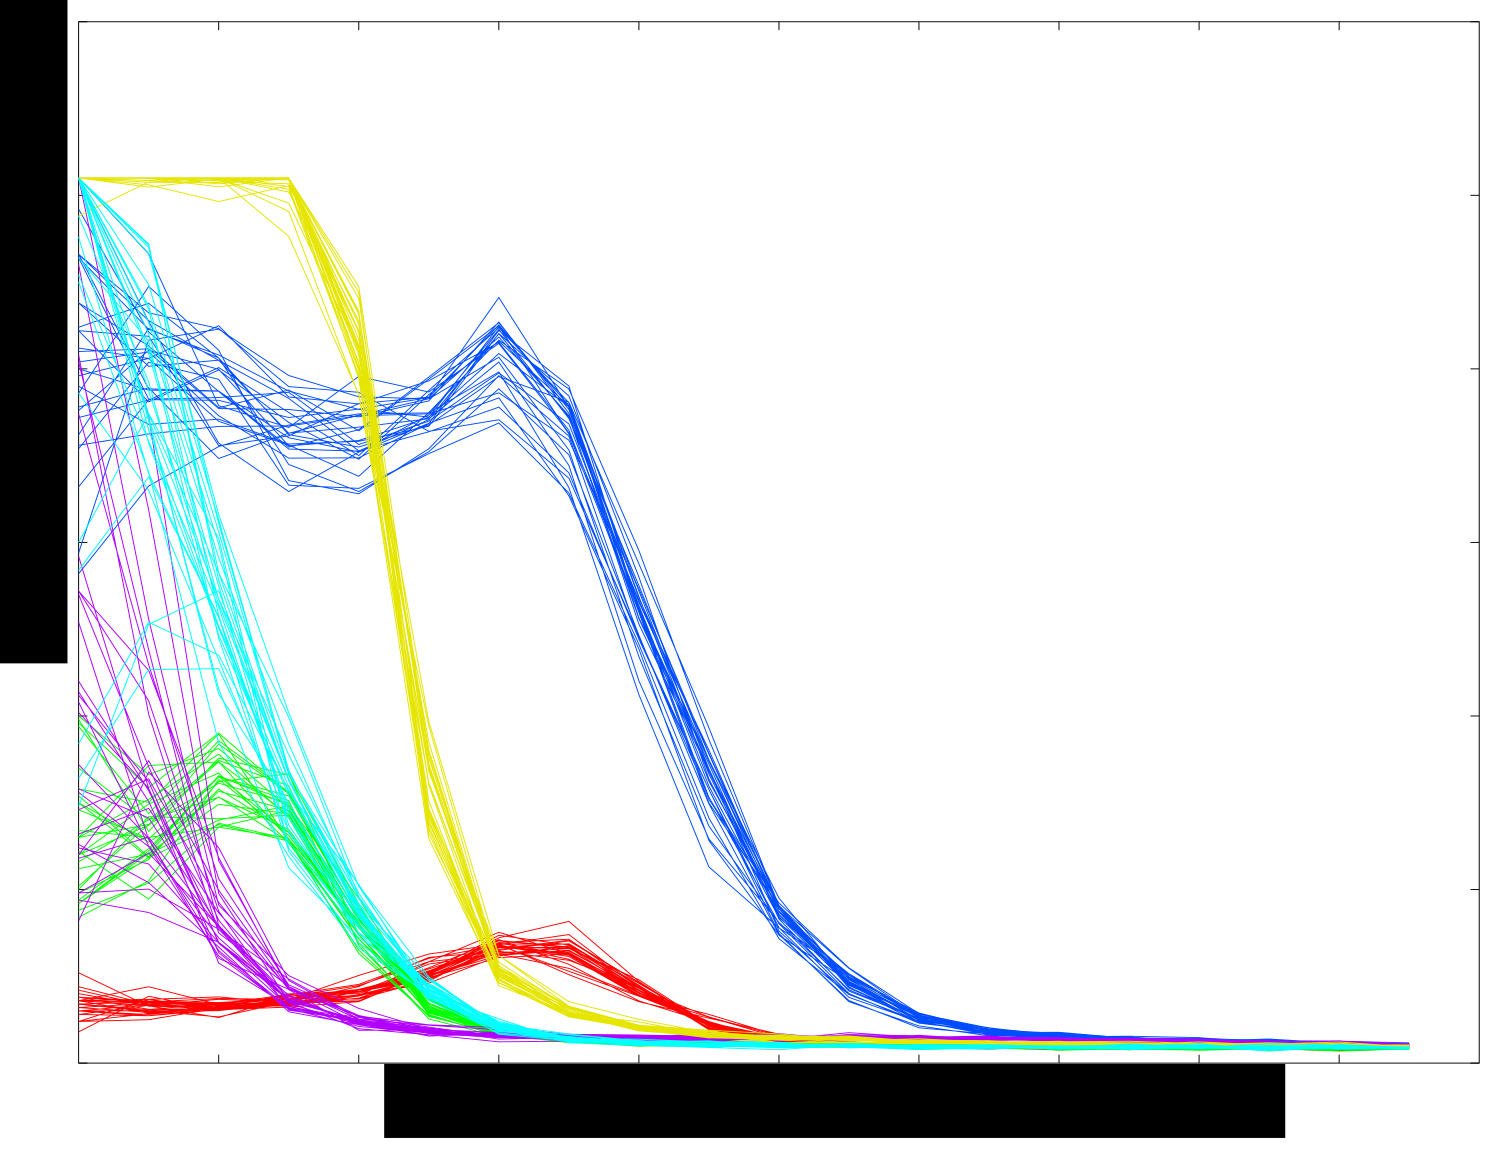
\includegraphics[width=0.99\linewidth]{images/AllLaserPersonalities_OneSpot.png}
\end{minipage}

\vspace{-0.1in}
  \caption{\label{figure:lasers} 
\textbf{Left:} False color renderings of the IR spill from  6
inexpensive green laser
pointers.  The pattern of this spill from a single laser is relatively constant, allowing
us to track and identify the lasers over time.  The pattern of spill
from the laser varies most with distance of the laser to the screen.
The top row of images were collected with the laser ~15 feet from the
screen, 
 the middle row was ~10 feet from the screen, 
and the bottom
row was ~5 feet from the screen. 
\newline
\textbf{Right:} This figure shows 30
  personality measurements for each of 6 lasers from a single
  calibration screen location. A single data point (a laser
  personality measurement) is represented by a radial histogram of
  intensities arranged by distance from the centroid of the laser
  spot, and each line represents one such data point. Each laser is
  represented by a different color. The intensity measurements range
  from 0 to 255 (y-axis), and the distances from the centroid of the
  laser spot range from 0 to 20 (x-axis). As an example, the blue
  laser's spot reaches its peak intense approximately 6 pixels from
  its center.
\vspace{-0.1in}
}
\end{figure}

% \fbox{CITE  Figure~!}

In addition to the centroid of the laser spot we extract the intensity
and size of the detected pixels to calibrate laser intensity data for
identification.  Inexpensive lasers exhibit a range of brightness and
focus, as shown in Fig.~\ref{figure:lasers} and this signature is
fairly consistent for each device.
% (once the laser has warmed up for about 15 seconds,
% and as long as the batteries are reasonably fresh). 
We call this intensity signature the laser's \textit{personality}.
During the calibration phase, we capture several frames' worth of this
intensity data at each of the calibration points for each laser.  We
observe spatial variation in the brightness and radius of the laser
spots due to the camera and projector lens and overall system angles
and geometry.  We examine the pixels of light and calculate a radial
histogram of the intensity values of the IR spot.
% In practice, 20 bins (representing a
% radius of 20 pixels) is sufficient to capture the uniqueness of a
% laser spot's shape. 
This intensity histogram acts as the laser's
personality.
% Note that the calibration can be performed simultaneously for many
% lasers (with 1 person per laser), and takes less than a minute.  The
% laser personality intensity calibration could also be performed
% passively and continuously, which we plan to explore in future work.
Sample personality data is presented in
Fig.~\ref{figure:lasers}.

% \fbox{CITE Fig.~\ref{figure:six_laser_personalities}!}


% \begin{figure}[t]
% \centering
% 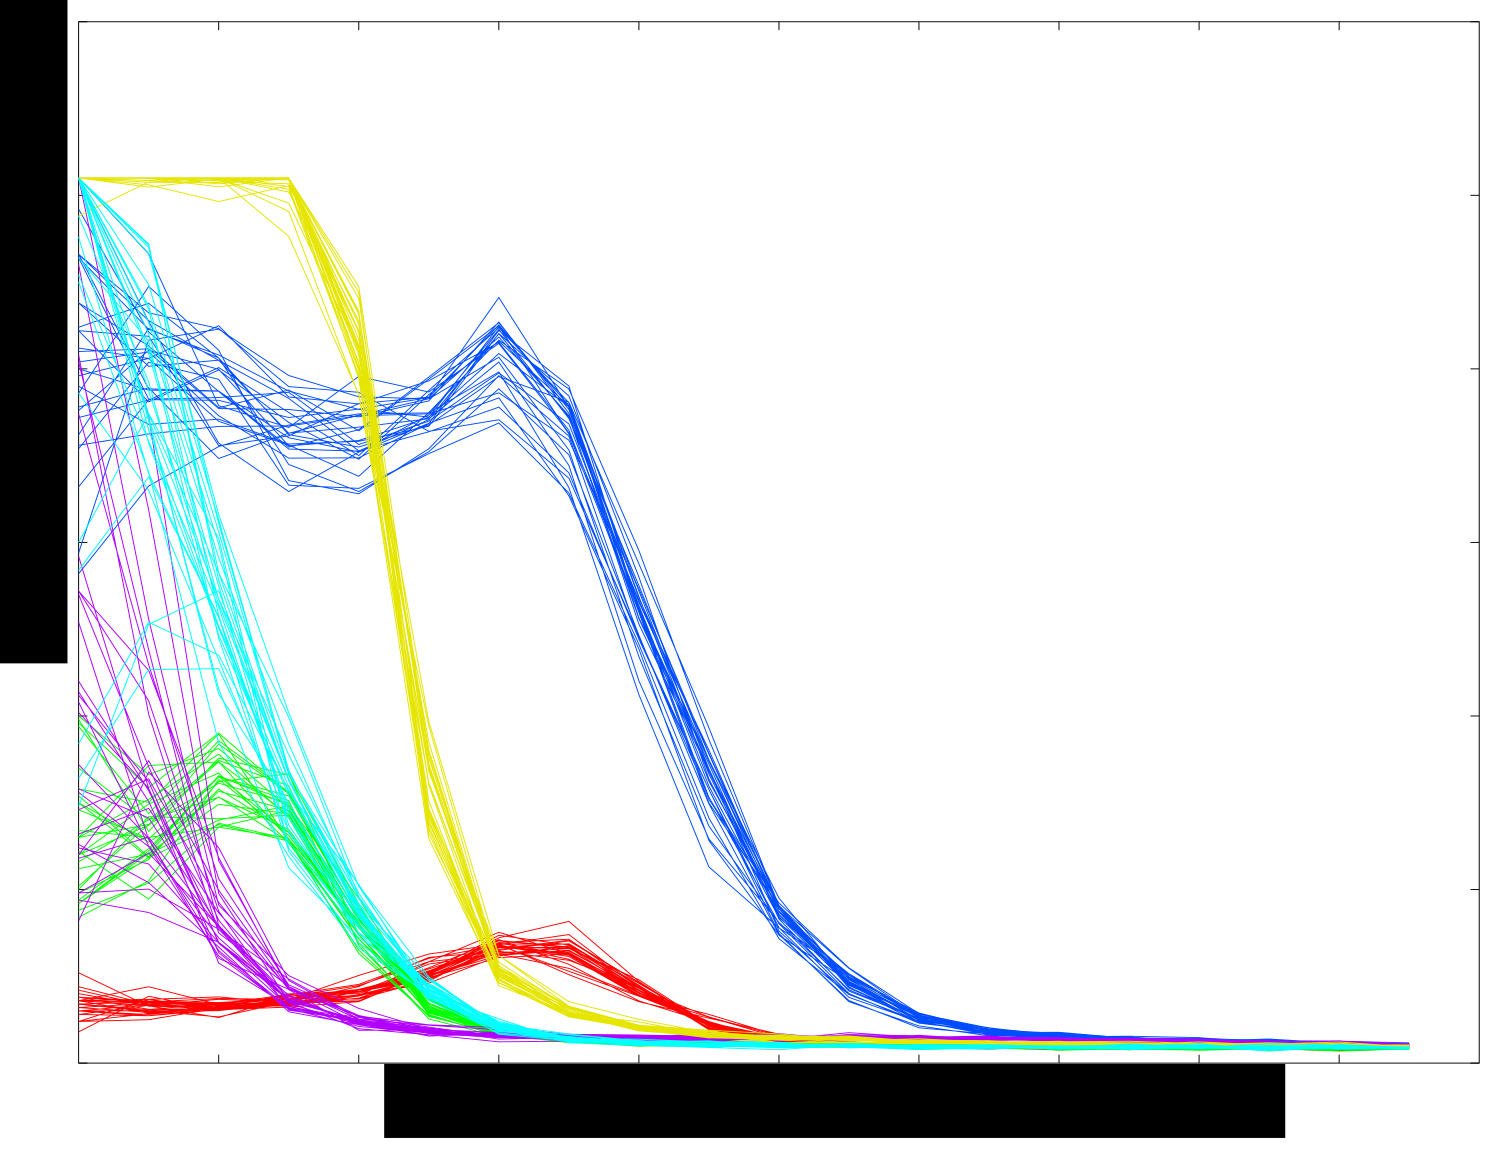
\includegraphics[width=0.65\linewidth]{images/AllLaserPersonalities_OneSpot.png}
% 
% \vspace{-0.1in}
% \caption{\label{figure:six_laser_personalities} This figure shows 30
%   personality measurements for each of 6 lasers from a single
%   calibration screen location. A single data point (a laser
%   personality measurement) is represented by a radial histogram of
%   intensities arranged by distance from the centroid of the laser
%   spot, and each line represents one such data point. Each laser is
%   represented by a different color. The intensity measurements range
%   from 0 to 255 (y-axis), and the distances from the centroid of the
%   laser spot range from 0 to 20 (x-axis). As an example, the blue
%   laser's spot reaches its peak intense approximately 6 pixels from
%   its center.
% }
% \end{figure}


% \subsubsection{Identifying Laser Spots: Matching Personalities}
% 
Once calibration is complete, the system is able to match any laser
spot on the projection surface with one of the calibrated lasers.
When a laser spot is detected, its personality is calculated, and
matched with that of one of the known lasers.
% 
% For efficiency, we utilize two passes to process the camera image.  In
% a first coarse pass, we examine every $n$th pixel in the camera image
% and all pixels greater than a pre-set intensity threshold continue to
% the second pass.  In the second pass, a generous window around each
% seed pixel is examined.  We collect all nearby pixels above the
% threshold and extract the largest connected component.  The centroid
% of this component is set as the laser spot position.  We then compute
% the histogram of pixel intensities shown in
% Fig.~\ref{figure:six_laser_personalities}.  
% The final task is to
% match the detected histogram to the library of known lasers.  
We do this matching by calculating the sum of squared differences
between the detected histogram and the histogram of each each known
laser.  We then assign the laser ID as the minimum of these sums.

% It is important to note that the apparent laser intensity varies
% spatially for each laser due to a number of additional variables,
% including: distance from laser to screen, distance from screen to
% camera, and camera vignetting.  We can easily normalize for these
% variations.  First, we normalize for the camera position by averaging
% all of the intensity data for all of the lasers collected at each of
% the calibration grid points, and normalize the input by dividing it by
% the spatial average.  We use barycentric coordinates and interpolation
% to normalize laser points between calibration grid locations.  Camera
% position normalization is especially crucial when the camera is placed
% at an extreme angle to the screen, and thus experiences significant
% perspective distortion.
% 
% 
% Just as the camera position relative to the screen is important, the
% laser spots also exhibit perspective distortion when they are used at
% extreme angle to the screen.  We can similarly normalize for this
% distortion, assuming that the intensity calibration data for each
% laser is collected from a position near that laser's use location.
% 
% \subsubsection{Temporal Coherence and Simultaneous Use}
% 
% For the tests presented in this paper and companion video we do not
% leverage temporal coherence in our detection.  Because the camera
% image and laser output contain some noise, the quality of the
% personality measurements and identification would benefit from
% averaging the output of multiple frames known to be the same laser
% from the tracking algorithm in Section~\ref{section:systemdetails}.
% 
% When multiple lasers are simultaneously detected on the screen, we can
% leverage this information to disambiguate lasers with somewhat similar
% histogram personalities.  We employ the Kuhn-Munkres algorithm to
% assign unique labels to all detected points; that is, no two lasers
% will be assigned the same ID, even if they both select the same ID as
% their first choice.

% We performed several tests to judge various notions of accuracy of the
% Laser Personality system. 
% % For results of these tests, please see Appendix \ref{appendix:accuracy_tests}. 
% These tests demonstrate that the laser personality
% system is very accurate when users are standing still, and acceptably accurate when
% they are moving around the room. This system is ideal for large-scale display setups
% in which many users can move freely and pass lasers off to one another while
% interacting with and exploring displayed data.

\vspace{-0.1in}

%%%%%%%%%%%%%%%%%%%%%%%%%%%%%%%%%%%%%%%%%%%%%%%%%%%%%%%%
\section{Conclusion}

\vspace{-0.1in}

%\fbox{what's a variable-scale display?  weird term}
%Multi-user interaction on variable-scale displays is a powerful
%collaborative tool with several applications.  


In this paper, we 
%have 
present
%ed 
a system for developing multi-user,
multi-cursor, multi-media, groupware that allows for intuitive
interaction with visual graph datasets.  The system's emphasis on
modularity facilitates extension to 
new input device types.
%additional include a variety of input devices
%(such as image-based 3D scanners) as new modules.  
Each separate input
module is treated as an abstract {\em cursor} that must adhere to
our set of common {\em gestures} for graph interaction.  This
abstraction is made possible by introducing an interface
%ing agent
between the application and the devices.
We will 
%be releasing 
open-source
our PolyMouse and Laser Personality systems.

Due to the nature of this modularity, a variety of input devices are
able to be included. 
% To allow our system to work with multiple input devices, and
% especially on large-scale projection surfaces with several mobile
% users, 
To include inexpensive green laser pointers as an 
%(a common groupware 
input device for
projection displays, we 
%have 
present
%ed 
a method for identifying
these lasers
%off-the-shelf laser pointers in an inexpensive and simple manner 
by calibrating each laser pointer's IR spillover's intensity
histogram, called the laser's \emph{personality}, allowing for
closest-neighbor matching of data points. 
% The inclusion of varied
%input methods allows for development for a variety of output devices
%beyond a simple PC monitor, including a large-scale projection surface
%as often seen in classrooms.

We 
%have 
demonstrate
%d
several visual graph exploration applications using this software
system to create intuitive and functional multi-user collaborative
experiences.  These applications take advantage of our 
%alternate 
automatic multi-user focus
and zoom 
algorithm
%level for multi-cursor collaborative interfaces, 
and demonstrate for
%its use on both large- and small- scale 
node-based
datasets.  Both our spatial data application (our utility
infrastructure groupware) and relational data application (our
collaborative data exploration groupware) take advantage of the system
by allowing multiple users to simultaneously explore, manipulate, and
visualize graph data while collaboratively problem solving using
simple gestures with either a mouse or a laser pointer, on both small-
and large-scale displays.



% 
% \fbox{section can be revised more to pull together more strongly the contributions and more.... }
% 
% In this paper, we present an effective method for accepting input from
% a variety of device types simultaneously.  We have demonstrated
% several visual graph exploration applications using this software
% system to create intuitive and functional multi-user collaborative experiences.
% %This allows for more efficient and possibly more inexpensive
% %collaborative learning experiences.  
% Our 
% %We have also presented a
% framework for groupware development takes advantage of our
% multi-device system to separate the groupware from the devices from
% which it is handling input. This is done by introducing an interfacing
% agent between the application and the devices that treats each device
% as an abstract {\em cursor} that makes {\em gestures} that are
% processed by the interface for the application.  
% This 
% %middleman
% abstraction results in cleaner, easier to debug, and extensible
% code.
% 
% We have also introduced an alternate focus zoom level for multi-cursor
% collaborative interfaces, and demonstrated its use on both large- and
% small- scale node-based datasets.
% 
% Finally, to allow our system to work with multiple input devices, and
% especially on large-scale projection surfaces with several mobile
% users, we have presented a method for identifying off-the-shelf laser
% pointers in an inexpensive and simple manner by calibrating each laser
% pointer's IR spillover's intensity histogram, called the laser's
% \emph{personality}, allowing for closest-neighbor matching of data
% points. 
% %The system requires only a calibration step to set up, and
% %once it is complete multiple users can interact with interfaces in a
% %large-scale environment.
% 
% Applications tailored to multi-user collaborative problem solving
% efforts are presented in this paper They take advantage of our
% system's ability to accept input from multiple device types and allow
% for efficient and collaborative node-based data exploration.

%
% %\vspace{-0.1in}
% %----------------------------
% \paragraph{\bf Future Work}


% our cursor and gesture software.
% \fbox{name drop our patented terms PolyMouse and laser personality system, but be consistent about capitalization}
%our system to the open source community, so that anyone may 
%download and develop applications for it.
%We will provide detailed instructions for setting up a system on your own to use
%multiple mice and laser pointers, as well as instructions for extending the system
%to work with other input devices.

% Our system is not without drawbacks, however. Extending it to include
% new input media, while straightforward, can be
% code-intensive. Recognizing gestures from media input is not a trivial
% task at times, depending on the complexity of the device.
% \fbox{vague, elaborate with interesting detail or cut}

% Crop zooming \fbox{Barb, drawbacks to Crop Zooming?}

%While 
The accuracy of our Laser Personality System is highest when
the  users do not change
their position relative to the screen (distance or angle).
While this is an acceptable requirement for lecture classroom use where students remain in their seats,
%which is
%sufficient for many applications, 
%how far they are from the projection
%surface does have an effect on the accuracy of the system, and
% (sufficient for many applications), 
%identification accuracy decreases if 
%there
%are times when this is not enough. 
% \fbox {reword previous sentence more... }
%
we would like to extend this work to 
%One clear extension to this work is the introduction of continuous
leverage continuous calibration during normal system usage.
% First, we will omit the special calibration step, and instead 
%We will generate initial calibration from early incidental usage, and
%continue to dynamically update a laser's data as it is used, replacing
%older calibration data as new data is read.
% As new data is added to the system, older data will be replaced, and so the calibration data will change as the 
% lasers' personalities do. This continuous update of the calibration data will allow for less confusion between 
% laser spots as the laser points warm up and change from continuous usage. 

%There are natural limitations to arise from using various hardware.
The accuracy of detecting our gestures is dependent upon
timing/detection sensitivity, which are in turn based on tolerances
that may vary depending on the resolution of the display, the user
skill, the application requirements, the speed of the processor, and
the size of the data.  Further analysis of these aspects of
development will be investigated with an in-depth user study.


% %
% \fbox{somewhere we need to discuss/mention the necessity of
%   timing/detection sensitivity in some of these gestures, and that
%   these timings and tolerances might vary depending on the resolution
%   of the display, the user skill, the application requirements, the
%   speed of the processor, the size of the data...  maybe this belongs
%   in future work...  user study...}

%----------------------------

% not necessary
% if accepted, we will acknowledge funding only

% \paragraph{Acknowledgments}
% Thank you to Andrew Dolce,
% % for his contributions to the laser-recognition code. Thank you to 
% Dr. W. Randolph Franklin, 
% % for his implementation of the least-cost flow routing hydrography method. Thank you to 
% Patrick Phipps,
% % for his work on 
% % the map visualization application and his graph data structure code, and thank you to 
% Andrew Zonenberg,
% % for his work on 
% % the map visualization application. Thank you to 
% Joshua Nasman, 
% % for his help with application testing, posing, and proof 
% % reading. Thank you to 
% Ryan Baltazar, and
% % for his ellipses-fitting code. Thank you to 
% Ted Yapo.
% % for his work on camera calibration.


% \appendix
% 
% \section{Laser Personality Accuracy Tests}
% \label{appendix:accuracy_tests}
% 
% The tests were performed using six
% lasers (given IDs 1-6) in the 19' x 23' space shown in Figure
% \ref{figure:laser_testing_room_diagram}. The space was divided into a
% series of testing locations, marked with an 'X' in the diagram, at
% discretized $22.5\,^{\circ}$ arcs with radii of 5', 10', and 15' from
% the center of the projection surface.
% 
% Two sets of calibration data were collected. For the first calibration
% (referred to from now on as calibration $C1$), all six lasers were
% calibrated from the 15' mark along the line perpendicular to the
% projection surface (point A in Figure
% \ref{figure:laser_testing_room_diagram}). For the second set of data
% (calibration $C2$), all six lasers were calibrated simultaneously from
% different points along the 10' arc (point B resides on this arc). The
% accuracy of a laser was defined as the percentage of frames in which
% the laser was identified correctly out of all detection frames. These
% results are presented in Table \ref{table:AccuracyTestingResults}.
% 
% %PLACEHOLDERS!
% \begin{figure}[t]
%   \centering
%   \includegraphics[width=0.65\linewidth]{images/room_diagram_annotated.png}
%   \caption{\label{figure:laser_testing_room_diagram} A diagram of the testing space. 'X's are marked in arcs at intervals of 5' 
% from the center of the projection surface, separated by $22.5\,^{\circ}$ arcs. Five locations (A through E) are marked on the diagram for reference. }
% \end{figure}
% 
% 
% \begin{table*} [t]
% \centering
% 
% \begin{tabular}{ | c | r | r | r | r | r | r | r | r | r | r | }
%  \hline
%  \textbf{Laser} & \multicolumn{2}{|c|}{\textbf{Single Pos.}} & \multicolumn{2}{|c|}{\textbf{Arc Mov.}} & \multicolumn{2}{|c|}{\textbf{Line Mov.}} & 
%                   \multicolumn{2}{|c|}{\textbf{Walking Path}} & \multicolumn{2}{|c|}{\textbf{All Lasers}} \\
%  \hline
%   1 & 100.00 & 100.00 & 96.54 & 98.27 & 53.88 & 74.14 & 51.13 & 68.49 & 99.79 & 100.00 \\
%   2 & 100.00 & 100.00 & 100.00 & 100.00 & 90.43 & 95.21 & 78.65 & 86.25 & 99.07 & 100.00 \\
%   3 & 95.85 & 100.00 & 70.96 & 73.48 & 35.14 & 48.65 & 60.50 & 96.10 & 83.49 & 98.75 \\
%   4 & 92.79 & 100.00 & 77.40 & 100.00 & 80.41 & 100.00 & 83.02 & 100.00 & 99.61 & 99.78 \\
%   5 & 99.67 & 99.67 & 100.00 & 100.00 & 57.99 & 92.57 & 82.95 & 94.26 & 99.80 & 99.92 \\
%   6 & 90.33 & 96.03 & 93.89 & 95.91 & 72.56 & 79.70 & 91.81 & 94.86 & 84.08 & 99.90 \\
%   \hline
%    & 521 & & 347 & & 230 & & 645 & & 968 & \\
%  \hline  
% \end{tabular}
% 
% 
% \caption{\label{table:AccuracyTestingResults}Results from accuracy
%   tests. Five tests were performed in all, and for each test and for
%   each laser two percentages are reported: the percentage of frames in
%   which it was correctly identified as its primary ID (left column), and the
%   percentage of frames in which it was identified as either the primary or secondary
%   ID (right column). The minimum number of frames collected for each test is reported
%   along the bottom row. All units are percentages of frames. }
% 
% \end{table*}
% 
% %During testing, a concerted effort was made to maintain a consistent
% %number of data collection frames within each test, and so 
% % The minimum number of frames considered for each test is reported in
% % Table~\ref{table:AccuracyTestingResults} along the bottom row. 
% Five
% accuracy tests were run in total, with users stationary, walking in an
% arc, walking along a straight line, walking along a path, and using
% all lasers simultaneously. For the tests, we count the number of times
% the laser is correctly identified as the primary choice, and the number of times the correct
% laser is either the primary or secondary choice (the laser intensity histogram with the
% next smallest sum of squared differences). These two values comprise
% the two columns in Table \ref{table:AccuracyTestingResults} for each
% test, with the primary ID on the left and the secondary on the right.
% 
% \subsection{Description of Tests}
% 
% The first four tests all used calibration data $C1$, while the final
% test used calibration data $C2$.
% 
% \textbf{Stationary Test} The purpose of this test was to judge how
% well lasers could be matched to the calibrated data. Data was recorded
% from the position at which the calibration $C1$ was collected,
% position A, and the tester did not move from that location. 
% % Each laser
% % was shone on the screen for at least 521 frames (roughly 17.75
% % seconds), making sure to point at both the middle and each of the four
% % corners of the screen. Each laser was correctly identified in at least
% % 90\% of the frames taken, and each laser was either identified
% % correctly or as the secondary laser at least 96\% of the time.
% 
% \textbf{Arc Walking Test} The purpose of this test was to judge how
% much side-to-side movement affected the overall accuracy of the
% identification system, because the shape of the laser spot is skewed
% when seen from an angle, changing the laser's personality. 
% Data was
% recorded while users walked along the 10' arc of data collection
% points, passing right-to-left through point B. 
% % The laser was kept as
% % close to the center of the screen as possible to avoid affecting the
% % laser spot in additional ways. Each of these tests lasted at least 347
% % frames (roughly 11.5 seconds). Four of the lasers performed well (with
% % at least 93\% accuracy), while lasers 3 and 4 maintained 70\%
% % accuracy. Each laser was identified as either its first or second
% % choice laser ID in at least 93\% of the frames, except laser 3.
% 
% \textbf{Straight Line Walking Test} The purpose of this test was to
% judge how much distance from the screen affected the overall accuracy
% of the system. 
% % Changing the distance to the projection surface changes
% % the radius and intensity of the laser spot, and thus affects the
% % histogram of the laser's personality. 
% For this test, the user stood as
% far from the screen as possible (approximately 20') and walked forward
% to the 5' mark, perpendicular to the screen.
% % The laser was once again
% % kept as close as possible to the center of the screen. Each of these
% % tests lasted at least 230 frames (roughly 7 seconds). The results for
% % this test were significantly poorer than other tests, as three of them
% % scored below 60\% (laser 3 scored below 40\%).
% % % This was the only test
% % %in which one of the lasers was more often identified as its secondary
% % %ID (laser 3) than its primary.
% 
% \textbf{Path Walking Test} The purpose of this test was to provide an
% overall averaging of the previous two tests, and to mimic movement
% expected by users in real-world environments. The path taken followed
% the letters marking room positions in Figure
% \ref{figure:laser_testing_room_diagram} from position A to B, C, D, E,
% and back to A. 
% % The laser was again kept as close as possible to the
% % center of the screen. Each of the tests lasted at least 645 frames
% % (roughly 19.5 seconds). In general, the lasers performed as expected,
% % an average somewhere between the arc and the straight line tests. Only
% % laser 1 fell below 60\% accuracy, while none of the other lasers beside laser 1 had more
% % than 15\% failure to be the first or second choice histogram
% % personality.
% 
% \textbf{All Lasers Simultaneous Test} The purpose of the final test
% was the assess how accurately the laser identification system
% performed when several lasers were on the screen at once. In this
% test, users stood at each of 6 marks along the 10' arc (the positions
% from which calibration $C2$ data was collected) and all shone lasers
% at the screen simultaneously. 
% % The laser spots followed a path that
% % touched all four corners as well as the middle of the projection
% % surface.  Two lasers, 3 and 6, were confused with one another in
% % approximately 15\% of the frames, but each of the other 4 lasers were
% % at least 99\% accurate.

\bibliographystyle{abbrv}
\bibliography{GD2013}


\end{document}

% The implementation of this feature is fairly straightforward.  
To prevent orientation confusion, the
re-focus and scale operations include a significant amount of damping
to prevent erratic scale and re-centering.
